\documentclass[11pt]{article}

\usepackage[margin=1in]{geometry}
\usepackage{booktabs}
\usepackage{amsmath}
\usepackage{hyperref}
\usepackage{graphicx}
\usepackage{xcolor}
\usepackage{tabularx}
\usepackage{ragged2e}
\newcolumntype{Y}{>{\RaggedRight\arraybackslash}X}

\title{Graphs 1--3: Missingness, Item Variance, and Row-Centring \\
\large Method and Artifact Report}
\author{DPCN Assignment 1 --- Opinion Network Formation}
\date{\today}

\begin{document}
\maketitle
\sloppy

\section{Scope and provenance}

This report documents three diagnostic figures built for the project:
missingness structure (Graph 1), item variance ranking (Graph 2), and the
empirical effect of row-centring (Graph 3). Their specification originated
from a ``Person 1 Work Packet'' document -- the same document family as the
untracked \texttt{data/temp.md} draft spec flagged earlier in this project,
which disagreed with the checked-in \texttt{CLAUDE.md} on several frozen
decisions (respondent filtering threshold, imputation statistic, which
network is primary). Rather than adopt that packet's pipeline wholesale, each
graph was built against numbers and artifacts verified directly against the
real CSV and against this project's actual, already-implemented pipeline
(\texttt{src/pipeline.py}), with any figure element that depended on the
rejected \texttt{>12}-missing filter corrected to reflect what this project
actually does instead.

\subsection{Artifact chain common to all three graphs}

\begin{center}
\begin{tabularx}{\linewidth}{l Y}
\toprule
Artifact & Role \\
\midrule
\texttt{data/Survey\_Results\_UC.csv} & Raw 96-respondent, 60-item source file \\
\texttt{src/loader.py} & Column parsing, missingness identification, Likert encoding \\
\texttt{src/imputation.py} & Ordinal logistic regression imputer (used by the pipeline, not re-run here) \\
\texttt{src/similarity.py} & \texttt{row\_centre()} and \texttt{compute\_spearman\_matrix()} \\
\texttt{src/pipeline.py} & Orchestrates loading, imputation, centring; produces \texttt{outputs/sanitised\_data/} \\
\texttt{outputs/sanitised\_data/} \newline \texttt{dataset\_imputed.csv} & Pipeline's exported, imputed, uncentred, 91-respondent matrix \\
\texttt{src/diagnostics.py} & New module holding all three graph-generating functions \\
\texttt{figures/} & Output directory for the three figures (PNG + PDF each) \\
\bottomrule
\end{tabularx}
\end{center}

\texttt{src/diagnostics.py} was written once and extended incrementally, one
function per graph. It does not duplicate pipeline logic: Graph 2 and Graph 3
read the pipeline's own exported CSV and call the pipeline's own
\texttt{row\_centre} and \texttt{compute\_spearman\_matrix} functions directly,
so their numbers are guaranteed to describe the same data the production
pipeline actually uses, not a parallel re-implementation that could silently
drift from it.

\section{Graph 1: Missingness map and response distribution}

\subsection{Purpose}
Characterise the raw missingness structure of the questionnaire before any
filtering, and demonstrate the acquiescence bias (grand mean well above zero)
that motivates row-centring later. This figure operates on the raw CSV
directly and does not depend on imputation.

\subsection{Artifacts used}
\begin{itemize}
  \item \texttt{data/Survey\_Results\_UC.csv} (input)
  \item \texttt{src/loader.py}: \texttt{load\_data}, \texttt{parse\_question\_columns},
        \texttt{identify\_missingness}, \texttt{encode\_responses}
  \item \texttt{src/diagnostics.py}: \texttt{plot\_missingness\_and\_response\_distribution}
  \item Output: \texttt{figures/graph1\_missingness\_response\_distribution.png/.pdf}
\end{itemize}

\subsection{Method}
\begin{enumerate}
  \item Load the raw 96$\times$61 file and parse the 60 item columns into
        codes (\texttt{T01}--\texttt{V15}) via their header-text prefixes.
  \item Encode Likert labels to $\{-2,-1,0,1,2\}$; any structural blank or
        literal \texttt{"No Comments"} becomes \texttt{NaN}. The resulting
        \texttt{encoded.isna()} mask is \emph{one} boolean missingness
        indicator covering both missingness mechanisms.
  \item Sum that mask per respondent (row), sort respondents descending by
        missing-item count.
  \item \textbf{Cutoff line}: rather than the work packet's \texttt{>12}
        threshold, the cutoff marks respondents with \emph{all 60 items
        missing} -- i.e. exactly what \texttt{src/loader.py}'s
        \texttt{drop\_entirely\_empty\_respondents} actually drops. Everyone
        else is retained and their missing cells are later filled by the
        ordinal regression imputer, not by a count-based exclusion rule.
  \item Left panel: the sorted boolean mask rendered as a two-colour image
        (dark = missing), with faint block-boundary lines at items 15/30/45
        and the cutoff drawn as a dashed line.
  \item Right panel: each respondent's own mean computed over only the items
        they answered (\texttt{skipna=True}); the 5 fully empty respondents
        produce \texttt{NaN} and are excluded from the histogram, since a
        mean over zero answers is undefined. A vertical line marks the grand
        mean, computed directly from the data rather than hardcoded.
\end{enumerate}

\subsection{Results}

\begin{center}
\begin{tabularx}{\linewidth}{l Y}
\toprule
Quantity & Value \\
\midrule
Total missing cells (raw, 96 respondents) & 542 (505 structural blank + 37 ``No Comments'') \\
Respondents dropped (fully empty) & 5 \\
Respondents retained & 91 \\
Missing cells among dropped respondents & 300 \\
Missing cells among retained respondents (to impute) & 242 \\
Missing rate among retained respondents & 4.43\% (242 / 5{,}460 cells) \\
Grand mean (all valid raw responses) & 1.138 ($\approx$ 1.14) \\
Sanity check: top sorted row's missing count & 60 / 60 (a genuinely empty respondent) \\
\bottomrule
\end{tabularx}
\end{center}

The 242-cell figure is not asserted independently -- it is cross-checked
against the pipeline's own reported \texttt{cells\_imputed} value in
\texttt{outputs/sanitised\_data/summary.json}, which is also 242. Both numbers
describe the same imputation step.

\begin{figure}[h]
\centering
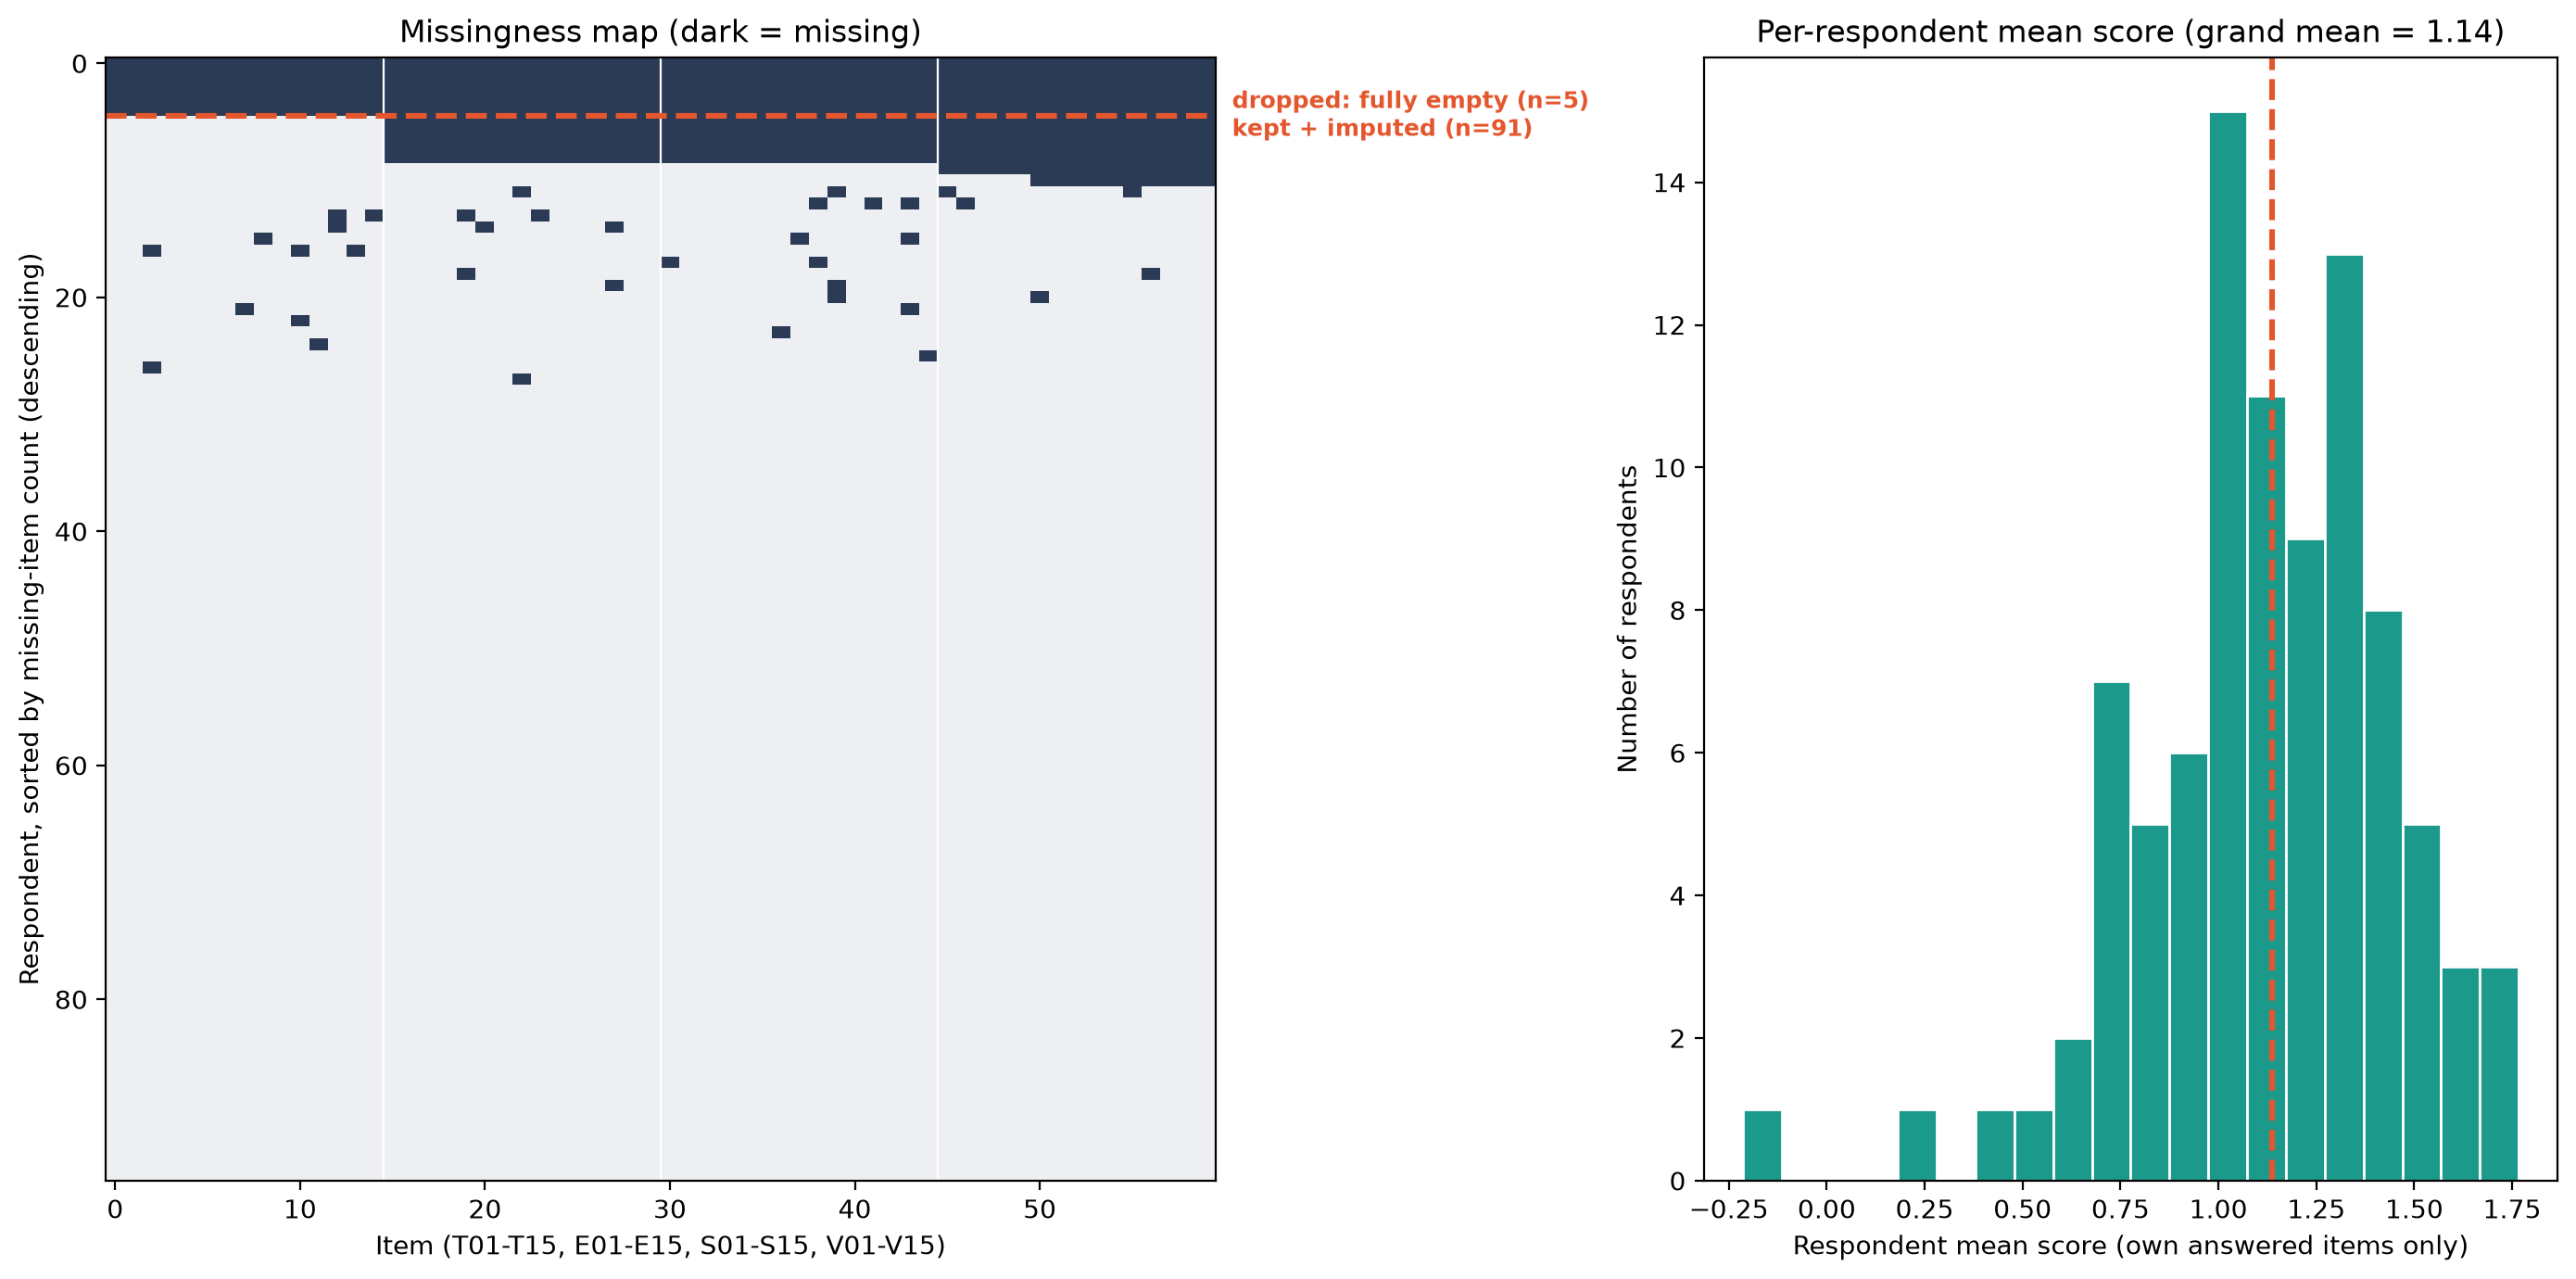
\includegraphics[width=\linewidth]{../figures/graph1_missingness_response_distribution.png}
\caption{Missingness map (sorted, dark = missing) and per-respondent mean
score distribution. The dashed orange line in the left panel marks the
actual drop boundary used by this project (fully-empty respondents only);
the dashed orange line in the right panel marks the grand mean.}
\end{figure}

\subsection{Deviation from the work-packet spec, and why}
The work packet's cutoff (\texttt{>12} missing items, producing 86 retained
respondents) was verified as internally consistent with the real data --
exactly 10 respondents exceed 12 missing items, carrying 495 of the 542
missing cells -- but this project's actual pipeline does not apply that
filter. Per an explicit decision made earlier in this project, only entirely
empty respondents are dropped; every other respondent, however incomplete, is
retained and imputed via a regularised ordinal logistic regression model
(\texttt{src/imputation.py}), not excluded by a missing-count threshold. The
figure was changed to show that decision rather than the packet's, since a
diagnostic figure should describe what the project actually does.

\section{Graph 2: Item variance ranking}

\subsection{Purpose}
Rank all 60 items by how divided respondents are on them, and check whether
contested/consensus items concentrate in particular topic blocks.

\subsection{Artifacts used}
\begin{itemize}
  \item \texttt{outputs/sanitised\_data/dataset\_imputed.csv} (input --
        the pipeline's own exported, imputed, uncentred matrix; not
        recomputed here)
  \item \texttt{src/loader.py}: \texttt{parse\_question\_columns} (recovers
        item codes from the exported header text)
  \item \texttt{src/diagnostics.py}: \texttt{plot\_item\_variance\_ranking},
        \texttt{BLOCK\_COLORS}, \texttt{BLOCK\_NAMES}
  \item Output: \texttt{figures/graph2\_item\_variance\_ranking.png/.pdf}
\end{itemize}

\subsection{Method}
\begin{enumerate}
  \item Load the pipeline's exported imputed matrix directly, rather than
        re-running imputation, so the numbers here are guaranteed identical
        to what the pipeline actually produced.
  \item Rename columns from full question text to item codes.
  \item Compute per-item standard deviation (\texttt{ddof=1}) on this
        \emph{uncentred} matrix. Row-centring is deliberately not applied
        here: it changes each item's variance and would answer a different
        question (spread after removing each respondent's personal baseline)
        than the one this graph asks (how divided is the class on this item,
        as actually asked).
  \item Sort items descending by SD; render as a horizontal bar chart, bars
        coloured by topic block using the same T/E/S/V palette already used
        elsewhere in the repository (\texttt{src/figures.py}).
\end{enumerate}

\subsection{Results}

\begin{center}
\begin{tabular}{lr}
\toprule
Quantity & Value \\
\midrule
SD range & 0.496 (\texttt{E15}) to 1.177 (\texttt{E04}) \\
Top 5 contested items & \texttt{E04, E03, E02, T08, T07} \\
Bottom 5 consensus items & \texttt{S11, S05, V06, V13, E15} \\
Mean SD, Technology block & 0.918 \\
Mean SD, Education block & 0.881 \\
Mean SD, Society/Ethics block & 0.794 \\
Mean SD, Environment block & 0.718 \\
\bottomrule
\end{tabular}
\end{center}

\begin{figure}[h]
\centering
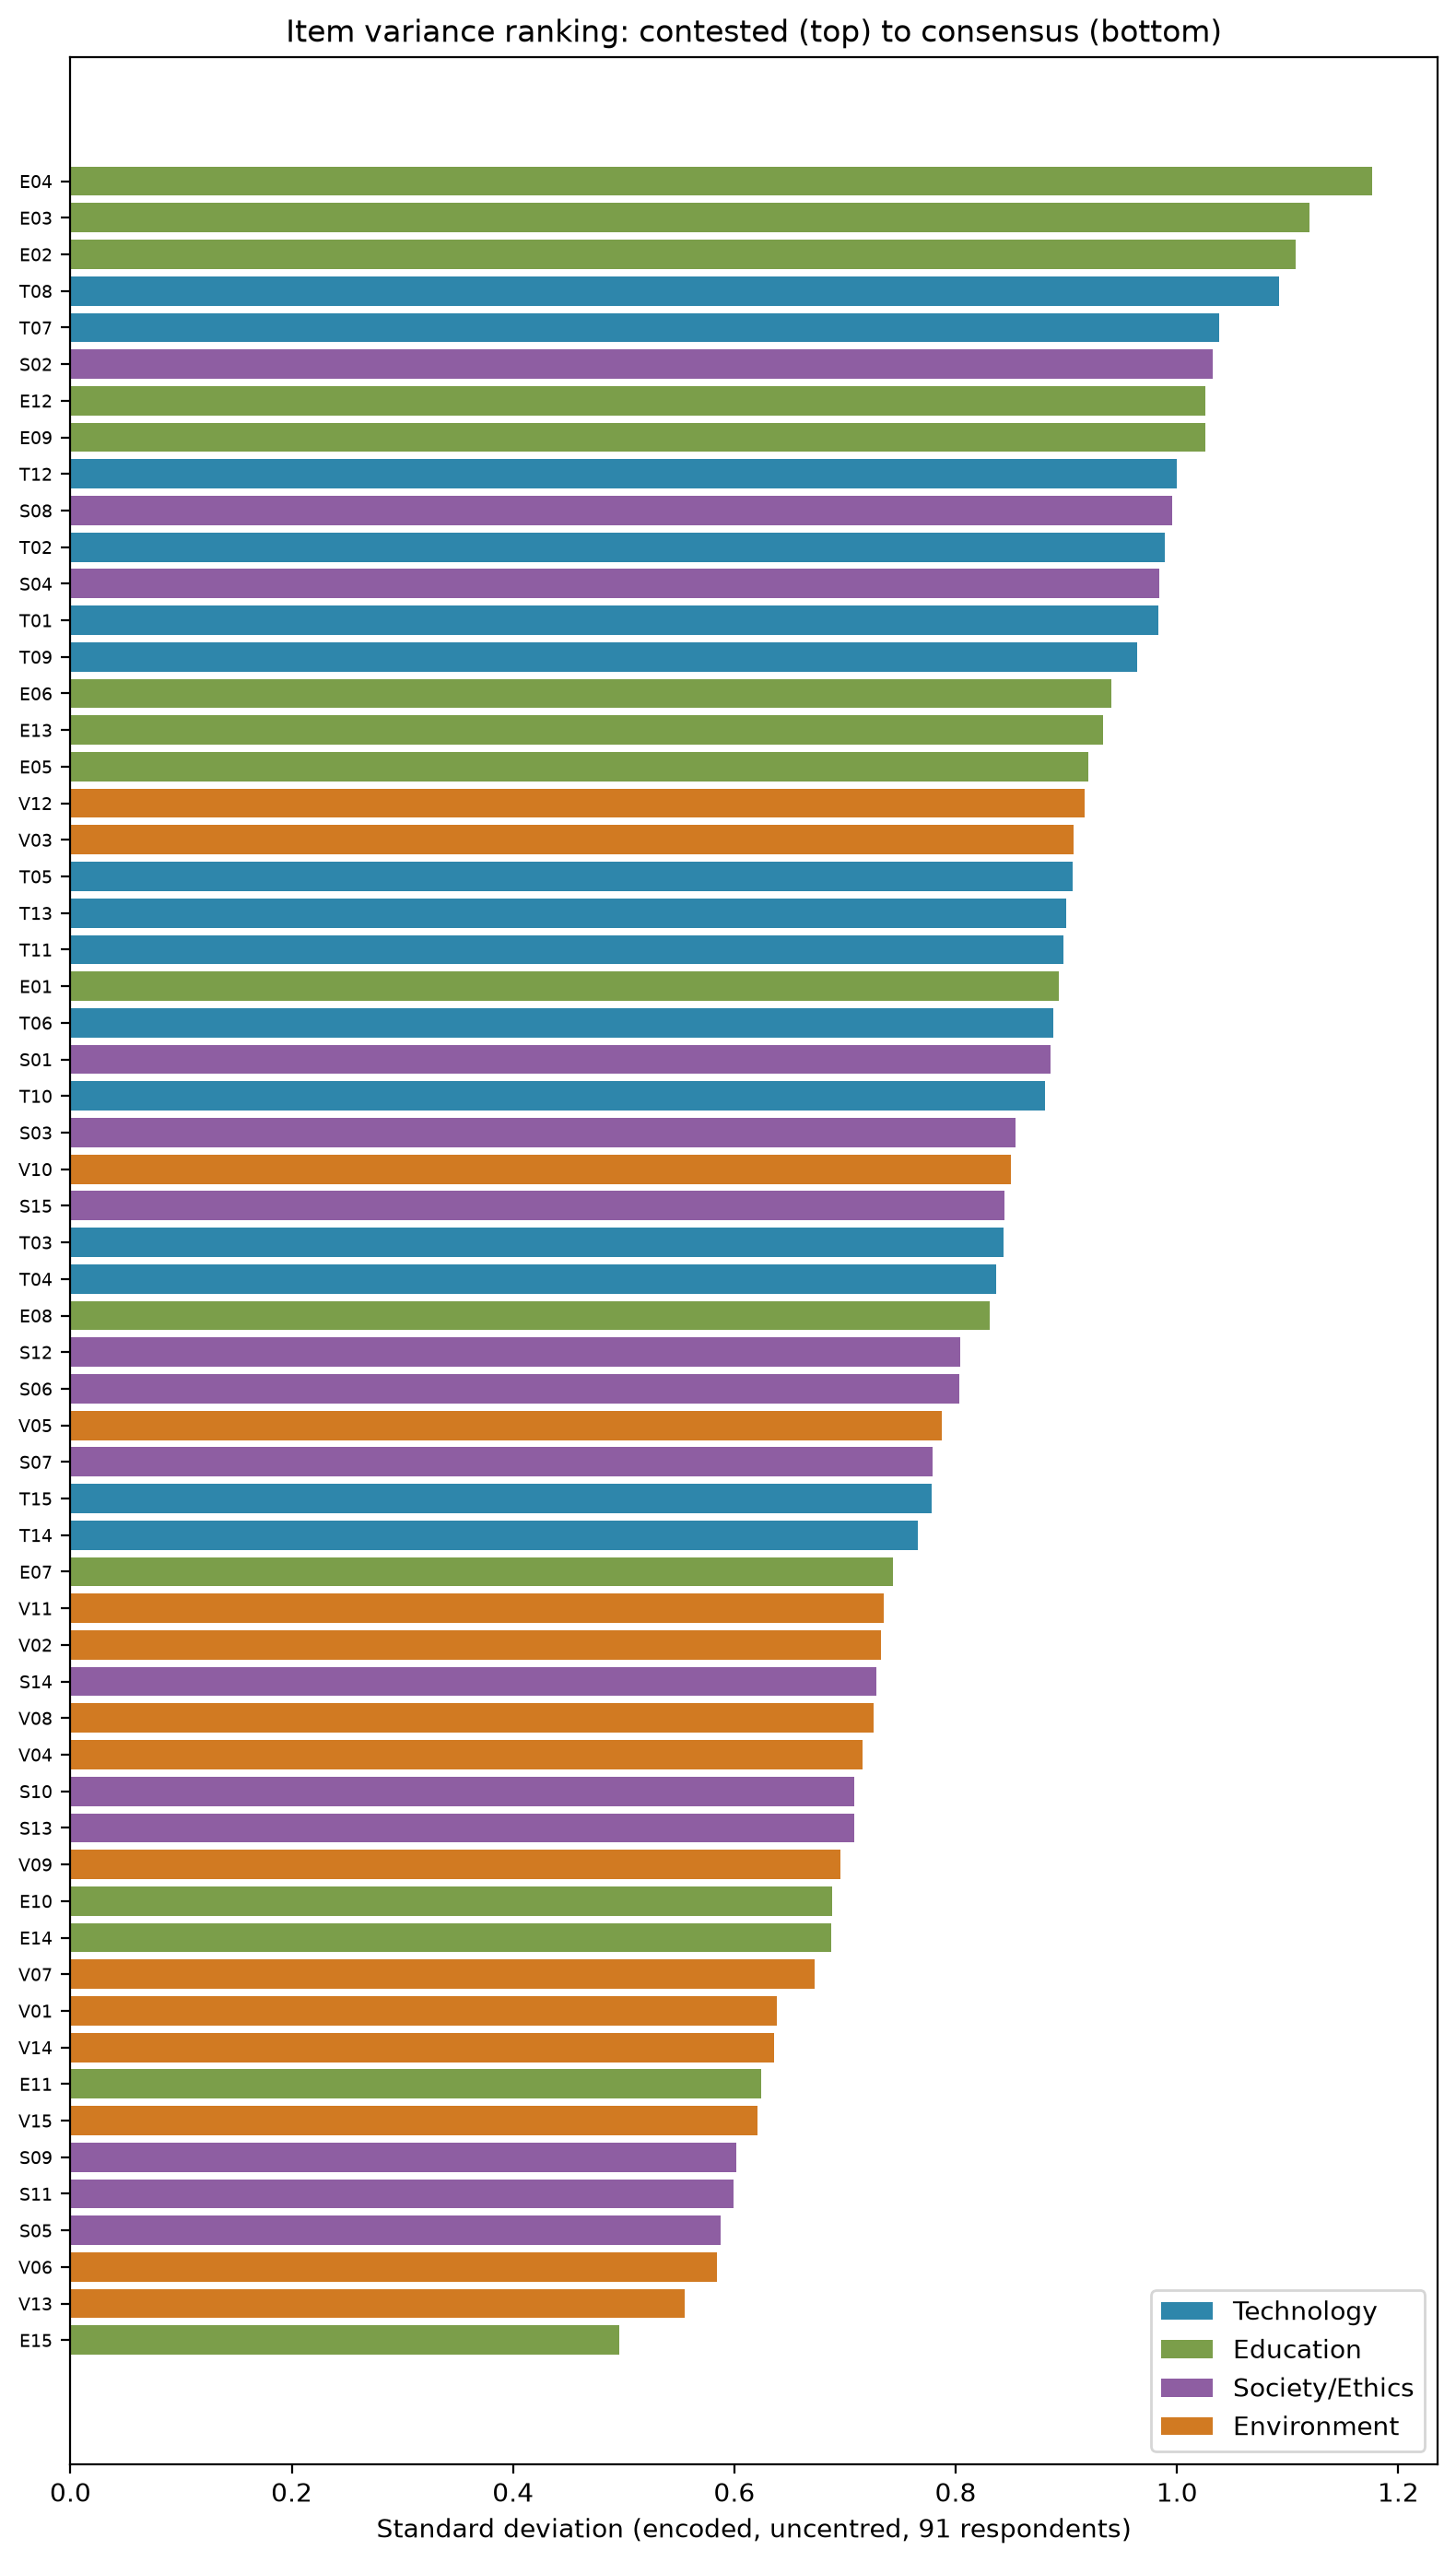
\includegraphics[width=0.75\linewidth]{../figures/graph2_item_variance_ranking.png}
\caption{All 60 items ranked by standard deviation, coloured by topic
block. Contested (top) to consensus (bottom).}
\end{figure}

\subsection{Finding}
Technology has the highest \emph{average} item SD (0.918), narrowly ahead of
Education (0.881). But the single most divisive individual items concentrate
in Education: three of the top five (\texttt{E04}, \texttt{E03}, \texttt{E02}
-- all about assessment and grading) are Education items, while Environment
supplies none of the top ten and two of the bottom five. This is a finding
about the survey instrument itself -- which topics have settled into
consensus versus which remain live disagreements -- not an artifact of
preprocessing, and is written up as such rather than only shown as a plot.

\section{Graph 3: Row-centring effect}

\subsection{Purpose}
Convert ``we row-centred the data because of acquiescence bias'' from an
assertion into a demonstrated, quantified effect on the actual correlation
structure used to build the item network.

\subsection{Artifacts used}
\begin{itemize}
  \item \texttt{outputs/sanitised\_data/dataset\_imputed.csv} (same input as
        Graph 2)
  \item \texttt{src/similarity.py}: \texttt{row\_centre}, \texttt{compute\_spearman\_matrix}
        -- called directly, not reimplemented, so this figure necessarily
        reflects the same transform and correlation method the production
        pipeline uses
  \item \texttt{src/diagnostics.py}: \texttt{plot\_row\_centring\_effect}
  \item Output: \texttt{figures/graph3\_row\_centring\_effect.png/.pdf}
\end{itemize}

\subsection{Method}
\begin{enumerate}
  \item Build the same 91$\times$60 item matrix as Graph 2, then row-centre
        it with \texttt{row\_centre()}.
  \item Compute the 60$\times$60 Spearman correlation matrix twice: once on
        the raw (uncentred) matrix, once on the row-centred matrix, using
        \texttt{compute\_spearman\_matrix} both times.
  \item Extract the upper triangle of each matrix
        ($\binom{60}{2} = 1{,}770$ pairs).
  \item Compute a single set of bin edges from the combined range of both
        distributions, and use those same edges for both histograms --
        directly addressing the spec's stated pitfall that mismatched bins
        make the visual comparison misleading.
  \item Plot both as overlaid, density-normalised histograms with vertical
        lines at each mean and a thin reference line at zero.
\end{enumerate}

\subsection{Results}

\begin{center}
\begin{tabular}{lrr}
\toprule
Quantity & Raw & Row-centred \\
\midrule
Mean $r$ & 0.151 & $-0.004$ \\
Median $r$ & 0.151 & $-0.008$ \\
Skewness & $-0.104$ & $+0.221$ \\
\bottomrule
\end{tabular}
\end{center}

\begin{figure}[h]
\centering
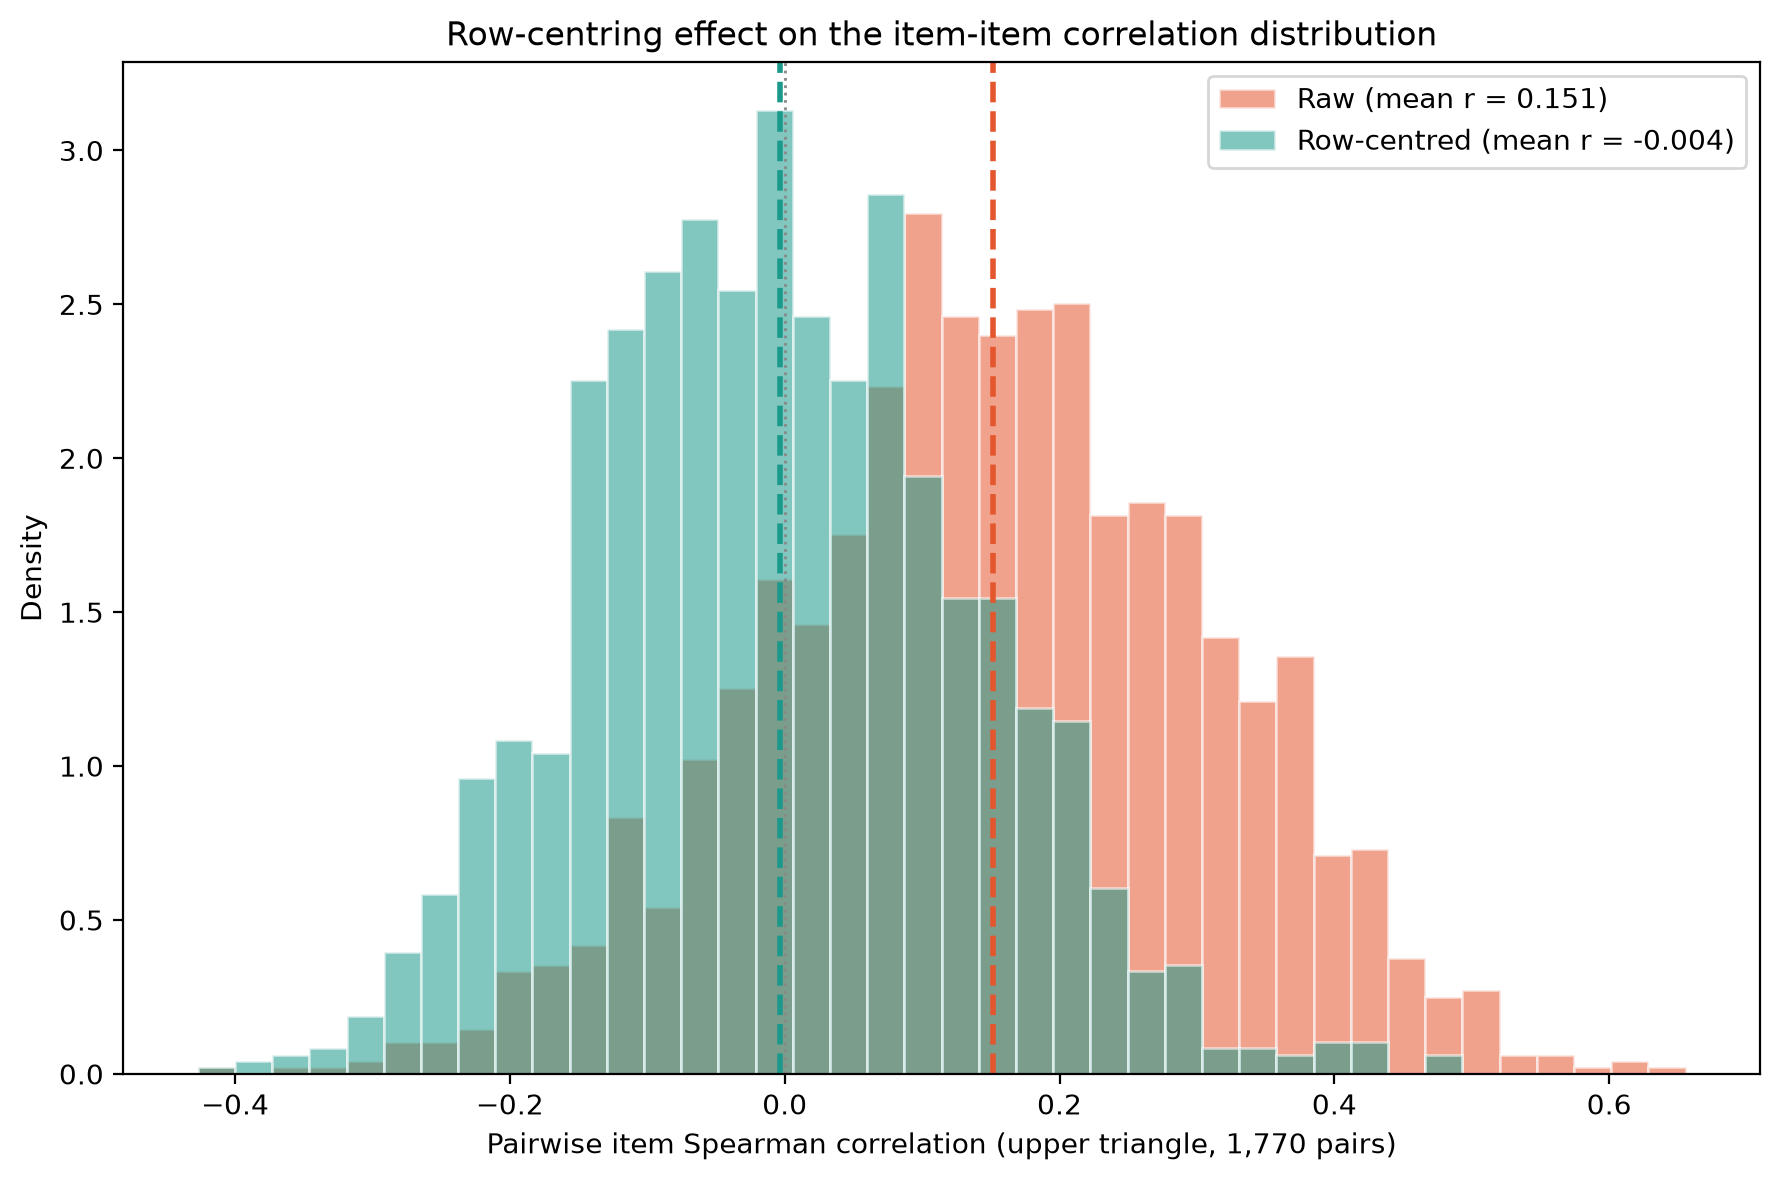
\includegraphics[width=\linewidth]{../figures/graph3_row_centring_effect.png}
\caption{All 1,770 pairwise item Spearman correlations, raw vs.\ row-centred,
on identical bin edges.}
\end{figure}

The raw distribution sits shifted positive (mean 0.151); the row-centred
distribution sits almost exactly on zero with a heavier right tail (positive
skew 0.221), matching the spec's predicted shape. The row-centred mean,
$-0.00377$, is an exact match to \texttt{weighted\_average\_correlation}
already recorded in \texttt{outputs/sanitised\_data/summary.json} -- confirming
this figure describes the identical correlation matrix the item network is
actually built from, not a separately-derived approximation.

\section{Cross-checks between graphs and the pipeline}

\begin{center}
\small
\begin{tabularx}{\linewidth}{Y Y Y}
\toprule
Number & Where computed here & Where verified against \\
\midrule
242 cells imputed & Graph 1 (\texttt{cells\_to\_impute}) & \texttt{summary.json}: \texttt{cells\_imputed} \\
$-0.00377$ mean centred $r$ & Graph 3 (\texttt{centred\_mean}) & \texttt{summary.json}: \texttt{weighted\_average\_correlation} \\
Grand mean 1.14 & Graph 1 (\texttt{grand\_mean}) & \texttt{CLAUDE.md}'s stated $+1.14$ \\
SD range 0.50--1.18 & Graph 2 (\texttt{min\_sd}, \texttt{max\_sd}) & \texttt{CLAUDE.md}'s stated 0.50--1.17 \\
\bottomrule
\end{tabularx}
\end{center}

None of these matches were forced; each was computed independently from the
underlying files and only then compared.

\section{Commit record}

\begin{center}
\begin{tabular}{ll}
\toprule
Commit & Contents \\
\midrule
\texttt{c8b9ac7} & Graph 1: missingness map + response distribution \\
\texttt{661133d} & Graph 2: item variance ranking \\
\texttt{eed3418} & Graph 3: row-centring effect \\
\bottomrule
\end{tabular}
\end{center}

All three were pushed to \texttt{origin/main}.

\end{document}
